\chapter{Introduction}\label{chap:intro}

\emph{“Our goal as computer scientist today, is to design the legacy systems of tomorrow.”}
\vspace{-1.5em}
\begin{flushright}
  \sidecite[][Timothy G.\ Griffin]{griffin2017legacy}
\end{flushright}

\margintoc%

\section{Context}

On the 1\nth{9} of July, 2024, 8.5 million Windows computers inside banks, airlines, TV
broadcasters, supermarkets and many other businesses suffered the infamous `Blue Screen of
Death' after (ironically) a faulty security update from cybersecurity
provider CrowdStrike was released.\sidecite[4\baselineskip]{verge2024crowdstrike}.

Even though it took only 78 minutes between when the issue was identified and
rectified, the ensuing chaos and disruption lasted hours if not days, as getting
the fix on affected machines and restarting complex systems was very difficult.
Although not as important as the human cost, the total financial cost in terms
of downtime for businesses was estimated by one insurer to be between 5 and 9
billion USD.\sidecite{fitch2024crowdstrike}.

To explain what went wrong, I need to outline some key concepts. An
\intro[OS]{operating systems} (OS), such as iOS, macOS, Windows or Ubuntu, is
the ``software you don't care about which runs the software you do care
about'', knowns as applications (`apps') or programs, such as a timer, a web
browser or a spreadsheet editor. It provides services to software, in a way
that abstracts from the details of the particular kind of hardware, for
example, the ability to respond to click from a mouse, or a tap from a touch
screen, or to play a sound via headphones or speakers. At the heart of the
operating system is the \intro[OS]{kernel} (for example Linux or Darwin for
Apple systems); it is the lowest level of abstraction within the operating
system. It uses the hardware via \emph{drivers} to provide key services like
deciding what gets to run (scheduling),and how much of the hardware it gets to
use (resource management), and protecting itself and other code from each other
(isolation).

As such, kernels are critical bits of a sometimes precarious tower of
abstractions, since they need to be both \emph{fast} \textemdash{} since any
latency here compounds throughout the whole computer \textemdash{} and
\emph{secure} \textemdash{} since any vulnerability here could crash or leak
data throughout the whole system. They are \emph{by necessity}, low-level
software, and need to be written in programming languages which expose lots of
control to the programmer, known as \intro{systems programming languages}.
However, more human control means more chance for human error. Historically,
this did not pose a multi-million computer, multi-billion dollar risk: both
hardware and software were much rarer, simpler and more trusted.

Cyber-security providers like CrowdStrike are written in \kl{systems
programming languages} and run at the kernel level\sidenote{A technically
questionable design choice, likely motivated by other factors.} to scan and
protect computers at a fundamental level, but this great power comes with great
responsibility, since, as we witnessed, the risks of an error is magnified
greatly at this level.

Whilst most of the commentary, including the root cause
analysis,\sidecite{rca2024crowdstrike} emphasised the need for better testing
and better deployment strategies, both of which are eminently sensible,
\emph{what} to test, and more importantly \emph{what's missing} in the tests
are only sufficiently clear with hindsight.

\emph{%
``The new IPC Template Type defined 21 input parameter fields, but the
integration code \ldots supplied only 20 input values to match against. This
\ldots evaded multiple layers of build validation and testing, as it was not
discovered during the sensor release testing process, the Template Type (using
a test Template Instance) stress testing or the first several successful
deployments of IPC Template Instances in the field.''
}

Aside from testing, Microsoft is also reported to be discussing locking down
access to the kernel with security vendors, and generally designing it to be
more robust to rogue drivers and updates.

To me, the situation seems akin to building a wall with Swiss cheese, and when
something gets through, saying `we should have had more layers' or `layers
designed this way'. Surely one might wonder if we can consider a less porous
material?

So far, the answer has been no: methods for improving the reliability of such
software are \emph{costly}, mainly in terms of expertise, but also in term of
time and effort, with little scope for critical \emph{ongoing} maintenance. And
whilst the exact contributions of this thesis would not have prevented
CrowdStrike (even hinting at that would be temeritous), they are extremely
relevant to the general domain.

This thesis argues that the answer is now a \emph{qualified yes}. A `less
porous material' is possible with what we know now, and not too complex
conceptually (though novel in its application). The main challenges come due to
\emph{scale}. Whilst the cost of the technology is still too high for mass
deployment, the trend is downward and should continue that way with sustained
effort.


\section{Thesis statement}

In this thesis, I will argue that building a verification tool for C, suitable
for handling low-level systems programming idioms, is two parts engineering,
and one part theory. Little of the theory are novel or complex, but its
application at scale present new challenges and insights. The proportions do
not correspond to three different topics, which fit neatly in either bucket.
Rather, each conceptual part of this thesis has varying mix of those
categories, which I will explain later in \nameref{sec:contributions}.

To put those parts into context, I first need to explain the role and quirks of
the venerable C programming language, and the relevant developments in
verification theory.

\section{The C programming language}\label{sec:c-lang}

More than fifty years after its introduction, and despite competition from
C++~\sidecite{isocpp1998} and Rust~\sidecite{rust}, C remains in common use. Part
of this is simply legacy: a lot of old and useful software is written in C.
However, most of this is the success C had in meeting its initial design goals:

\begin{itemize}
    \item \textbf{Portability}. C was designed to have a relatively small set
        of defined behaviours, leaving several key choices as
        \intro[UB]{undefined behaviour}s (UBs). This allows C programs to
        exploit the advantages of several different kinds of hardware to run
        quickly.
    \item \textbf{Simplicity}. C was designed to be concise and simple to
        compile (in one pass if need be), so that it was relatively
        straightforward to write C compilers to support new hardware.
    \item \textbf{Proximity to hardware}. C was designed to be a `portable
        assembly', close to hardware, so that the programmer had precise
        control over the resources used (especially when CPUs were much slower
        and memory far more constrained).
\end{itemize}

As time went on, hardware became faster, by becoming more complex and so C's
proximity to it waned. However, it continued to be used in performacne critical
code such as the Linux \kl{kernel}. Portability, assisted by a large set of
\kl{UB}, became avenues for optimisations. Under pressure for faster code,
simplicity of compilation gave way to complex alias analysis and pointer
provenance reasoning to optimise code.

\begin{marginfigure}
    \centering
    \cfile{code/pointer_from_integer_1pg.c}
    \caption{Example pointer\_from\_integer\_1pg.c.}\label{fig:ptr-from-int-ub}
\end{marginfigure}%

\cref{fig:ptr-from-int-ub} shows a slightly contrived example (courtesy
of~\sidetextcite{memarian2019exploring}), which nevertheless illustrates the
alias assumptions at play here. It assumes that \cinline{ADDRESS_PFI_1PG} is
the guess the address of a variable local to function \cinline{f}, which is
cast to a pointer in \cinline{main}, and then passed in as an argument to
\cinline{f}. The question this raises is: even if the guess matches the runtime
address of the local variable, should the compiler be allowed to assume that
pointers passed in as arguments cannot alias local variables? From a purely
concrete point of view of pointers (they are simply numbers), the answer is no,
yet this would disable constant propagation in the printed value in this
example.

\begin{marginfigure}
    \centering
    \cfile{code/pointer_from_integer_1ie.c}
    \caption{Example pointer\_from\_integer\_1ie.c.}\label{fig:ptr-from-int}
\end{marginfigure}%

However, the other extreme, of assuming pointers are purely symbolic and always
non-aliasing is definitely incorrect in C, because of C's ability to
\emph{compute} with pointers (increment, calculate offsets, cast them to and
from integers). An example similar to the previous one (from the same source)
is shown in \cref{fig:ptr-from-int}, with the difference that instead of the
address being cast to a pointer in the calling function \emph{before} the local
variable is in scope one, it is cast to a pointer \emph{after} and its address
has been variable is \intro{exposed}: cast to an integer (but otherwise
unused). Though we can clearly see that there is no dataflow beteween
\cinline{k} and \cinline{i}, in general, the compiler cannot rule it out, so it
conservatively disables constant propagation to the call to \cinline{printf}
later.

Stakeholders have attempted to resovle such questions by the formation of and
continual updates to the \kl{ISO} standard of C,\cite{isoC1990} however, the
resolutions can be complex and subtle. This is because of the different
preferences for performance, control and language simplicity, amongst
application programmers, systems programmers and compiler writers. To add to
the confusion, as a prose English document, the standard has some irreducible
ambiguities, and does not necessarily reflect \intro{de facto} C, as is it
used in practice, so even memorising the standard would not be enough to
safeguard against unexpected language quirks.

Given this state of affairs, the \intro{Cerberus}
project~\sidecite{memarian2022cerberus} aims to provide a formally defined,
executable and \emph{empirically validated} semantics of C, both ISO and \kl{de
facto}. We shall explain Cerberus' particular advantages over other tools in
\cref{sec:cerberus-core}. For now, it suffices to say that Cerberus works by
\emph{\kl{compositional}ly} elaborating C into a first-order functional
language (known as `\intro{Core}') with a few purpose-built constructs. It
makes explicit many implicit quirks of C such as integer promotion, \kl{UB} and
loose evaluation order.

The \intro{compositional} nature of in particular allows a user to see how the
elaborated \kl{Core} relates to the C a user wrote. I will use a function which
appends singly-linked list of integers to another as a running example.

\begin{marginfigure}
    \centering
    \cfile[breaklines]{code/append_plain.c}
    \caption{Singly-linked integer list append in C.}\label{fig:append-c}
\end{marginfigure}%

In this (admittedly unidiomatic) example, \cinline{NULL} pointers represent
empty lists, and so the function returns \cinline{ys} if \cinline{xs} is empty,
otherwise it recurses on \cinline{xs->tail} to get the new tail
\cinline{new_tail} and sets \cinline{xs->tail} to point to that,  returning the
result as \cinline{xs}.

This is elaborated into \kl{Core} (\cref{fig:append-core}). All the
subtleties and sources of \kl{UB} in C, including signed integer over/underflow,
use-after-free, leaking, and double-free memory management errors,
\kl[OOB]{out-of-bounds} indexing in arrays, and dereferencing a \cinline{NULL}
pointer. These form the contract between the compiler and the programmer, and
violations can result in difficult to debug, and costly mistakes. From the
perspective of the compiler, they are \emph{assumptions about the program and
its execution}, and so ideally be \emph{proven} absent; they are not things one
can check by running the program (though there are tools which instrument code
in various ways can find such errors, CN included). To aid programmers in
proving such \kl{UB} absent, we must understand how we can prove things about
imperative, memory manipulating programs.

\section{Verification with Separation Logic}

The key ideas around proving properties about imperative programs originate all
the way back towards the end of the 1960s, with~\citeauthor{floyd1993assigning}
and~\citeauthor{hoare1969axiomatic}. The basic setup is a triple of
$\{P\} \;C \; \{Q\}$, where $P$ is a \intro{precondition}, a predicate describing the
intial state of the program; $C$ is the program which executes; and $Q$ is
\intro{postcondition}, a predicate describing the final state of the program.
Combined with a set of inference rules to construct proofs from smaller parts
of $C$, this gave programmers a way to do pen-and-paper proofs about the
behaviour of imperative programs.

This approach works well enough, up until the programming language introduces
support for potentially aliasing pointers, at which it becomes
unfeasible.\sidenote{This and the following two paragraphs rely heavily on the
explanation of \textcite{pichon2017hlogmodc}.} In short, the issue is that
whilst assertions in the specification language might \emph{syntactically}
refer to different locations, \emph{semantically} those locations may alias,
thus breaking the rule of constancy (\cref{fig:rule-of-constancy}). This rule
is critical for \intro{modular} verification for programs because we can use it
to glue togethter two separately verified programs, and compose them (e.g.\
sequentially) so long as they refer to separate program variables.

\begin{marginfigure}
  \begin{mathpar}
      \inferrule{\vdash{} \{P\} \; C \; \{Q\}  \\ \mod{(C)} \cup{} \mathit{FV} (R)}
                {\vdash{} \{ P \wedge{} R \} \; C \; \{ Q \wedge{} R \}}
  \end{mathpar}
  \caption{The rule of constancy, where $\mathrm{FV}$ refers to the free
      variables of an assertion and $\mod{}$ is a syntactic
      over-approximation to the set of program variables a program might
      modify. It states that \kl{precondition}s which do not refer to mutated
      program variables remain true that program terminates.}\label{fig:rule-of-constancy}
\end{marginfigure}

To prevent this, we would have to use the following rule, which requires the
pre- and postconditions to mention $E_3$ and $E_4$ even though they are not
mentioned syntactically in $ [ E_1 ] \mathbin{{:}{=}} E_2$, so that the
non-aliasing condition $E_1 \noteq E_3$ can be stated, and the morally disjoint
fact $E_3 \hookrightarrow{} E_4$ is preserved into the postcondition.%
\[
    \inferrule{}{\vdash{}
        \{ \exists{} v.\ E_1 \hookrightarrow{} v \wedge{} E_1 \noteq E_3 \wedge{} E_3 \hookrightarrow{} E_4 \}
        \; [ E_1 ] \mathbin{{:}{=}} E_2 \;
        \{ E_1 \hookrightarrow{} E_2 \wedge{} E_3 \hookrightarrow{} E_4 \} }
\]

This scales poorly: composing one program with $n$ variables and up to $O(n^2)$
no-aliasing conditions, with another program of $m$ variables and up to
$O(m^2)$ leads to new assertions with up to ${O(n + m)}^2$ conditions. The
problem is bad enough that the design of the verification-oriented Euclid
programming language put in place several restrictions to prevent aliasing in
the language, unlike its main influence, Pascal, which permitted
it.\sidecite{popek1977notes}

The key breakthrough came with the arrival of separation logic by John C\@.
Reynolds and Peter O'Hearn.\sidecite{reynolds2002separation} Specifically, the
introduction of the \intro{separating conjunction}, $\astRef$, allows us to
state a version of the rule of constancy which is sound, known as a the
\intro{frame rule} (\cref{fig:frame-rule}). Not only did this enable the
practical pen-and-paper verification of programs with pointers, aliasing, and
dynamic memory management, it was very soon extended to aid in reasoning about
several types of concurrency and is now mechanised in a very general way in
proof assistants~\cite{jung2018iris, appel2011verified}, enabling complex
proofs about large and subtle systems.

\begin{marginfigure}
  \begin{mathpar}
      \inferrule{\vdash{} \{P\} \; C \; \{Q\}  \\ \mod{(C)} \cap{} \mathit{FV} (R)}
                {\vdash{} \{ P \ast{} R \} \; C \; \{ Q \ast{} R \}}
  \end{mathpar}
  \caption{The frame rule. We still need to be careful about non-intereference
      about program variables on the stack, so we retain $\mod{(C)} \cup{}
      \mathrm{FV}(R) = \emptyset{}$, but locations on the heap are ensured
      disjoint by the definition of $\astRef$. The name comes from the
      \emph{frame problem} in artificial intelligence, where using first-order
      logic to represent the world requires many axioms simply to state that
      things do not change arbitrarily.}\label{fig:frame-rule}
\end{marginfigure}

To conclude this section, I will continue the example of appending to a list,
but this time in separation logic, in a simple imperative language. It says
that expression $\mathsf{i}$ is either $\mathsf{NULL}$ and thus represents an
empty list in memory, or there exists an integer $v$ and list $l'$ and location
$\mathsf{j}$ such that $l = v {:}{:} l'$, $\mathsf{i}$ points to $v$, its
adjacent cell $\mathsf{i}+1$ points to $\mathsf{j}$ and the list predicate
holds recursively for values $\mathsf{j}$ and $l'$. In this way, it relates the
contents of linked heaps cells, laid out in a particular format, to a
mathematical list \intro{ghost} value, which exists only in the specification
of the program but not in the runtime.

\begin{marginfigure}
    \centering
    \begin{align*}
        \mathrm{list} &(\mathsf{p}, l) \mathrel{{=}^\mathrm{def}} \\
                      &\mathsf{emp} \astRef{} (\mathsf{p} = \mathsf{NULL} \wedge{} l = []) \\
                      &\vee{} \exists{} \; {head}, \; {tl}, \mathsf{p\_tail}.\\
                      &\qquad l = {head} {:}{:} {tl} \\
                      &\qquad \astRef{} (\mathsf{p} \mapsto{} {head}) \\
                      &\qquad \astRef{} (\mathsf{p} + 1 \mapsto{} \mathsf{p\_tail}) \\
                      &\qquad \astRef{} \mathrm{list} (\mathsf{p\_tail}, {tl})
    \end{align*}
    \caption{Definition of a recursive list predicate in a simple separation
        logic.}\label{fig:list-pred}
\end{marginfigure}

With the predicate in \cref{fig:list-pred}, we can write a proof sketch of a
version of the list \mintinline{text}{append} program from \cref{fig:append-c},
with intermediate assertions inserted (\cref{fig:append-annot}). Because the
definition \mintinline{text}{append} is recursive, we annotate it with a pre-
and postcondition, and prove that the implementation matches it (assuming it
holds at structurally smaller values). The precondition states we start with
two disjoint heaplets representing two \kl{ghost} lists,
$\mathrm{list}(\mathsf{xs}, l_1)$ and $\mathrm{list}(\mathsf{ys}, l_2)$, and
the postcondition says that the value returned by this function
($\mathsf{ret}$) represents the concatenation ($@$) of the two logical lists
from the input.

Under the true-branch of the \mintinline{text}{if}, we have that $\mathsf{xs} =
\mathsf{NULL}$ and so it represents the empty heap, meaning the return value
and associated \kl{ghost} list is simply $\mathsf{ys}$ and $l_2$ respectively.
Under the false-branch, because $\mathsf{xs} \noteq{} \mathsf{NULL}$, we may
assume we can unroll the definition of $\mathrm{list}$, before calling
\mintinline{text}{append} recursively on the smaller
$\mathrm{list}(\mathsf{xs}', l_1')$, which allows us to conclude
$\mathrm{list}(\mathsf{new\_tail}, l_1' @ l2)$. Using the frame rule, the
$\mathsf{xs} \mapsto v \astRef (\mathsf{xs} + 1) \mapsto \mathsf{xs}'$ remains
unchanged and so we can fold these components into $\mathrm{list}(\mathsf{xs},
l_1 @ l_2)$.

\begin{marginfigure}
    \inputminted[breaklines,mathescape,fontsize=\small]{py}{code/append_annot.py}
    \caption{A separation logic proof sketch of a singly-linked integer list
        append.}\label{fig:append-annot}
\end{marginfigure}

Whilst very useful, and certainly a huge leap forward based on what was
available before, this example also highlights the limitations of the
traditional approach. It works over an idealised imperative language, suitable
for simple proofs of algorithms and their implementations, and the link between
this and the C implementation in \cref{fig:append-c} is based on trust. This
issue persists with contemporary, mechanised frameworks for separation
logic,\sidecite{appelSF5,sammler2021refinedc,jacobs2011verifast}
which use trust-based model of C, rather than an \emph{empirically validated}
one.

\section{CN:\ C, No bugs!}\label{sec:cn-intro}

\intro{CN},\sidenote{`\kl{CN}' does not stand for anything; its name is a
historical accident, though the backronym in the section title was suggested by
Elizabeth Austell.} in its \intro{proof mode}\sidenote{There are other modes to
\kl{CN}, most notably instrumentation and test generation, which I will mostly
ignore.} is a verification tool whose aspirational goal is to lower the cost of
C verification from a Rocq~\sidecite{CDT2024} programmer who knows separation
logic to a systems programmer who knows Haskell~\sidecite{haskell}.\sidenote{This pithy wording is
courtesy of Neel Krishnaswami.} It is designed to be used pre-existing C
programs (so they are not written or structured in a way to be verified
beforehand). Before I explain how \emph{works}, I will first explain how it is
\emph{used}.

When given a C file, \kl{CN} ensures that (a) the input code is free of
undefined behaviour and (b) correctly implements any specification written in
\intro{annotations} in comments with an @ symbol \cinline{/*@..@*/}
(so that they are first and foremost, for almost all C tools, a regular C
comment). Importantly, for compositionality, performance (paralellisability),
and ease of annotation,\sidenote{Annotations follow the structure/units of the
program.} these are checked on a \intro{per function} basis.

This means that even in the absence of annotations, code is being checked for
undefined behaviour. Incrementing an unsigned integer is perfectly acceptable
(\cref{fig:un-incr}) but incrementing a signed integer triggers an error message
(\cref{fig:incr-broken}).

\begin{marginfigure}
    \centering
    \cfile[breaklines]{code/unsigned_increment.c}
    \caption{Unsigned integer increment in CN.}\label{fig:un-incr}
\end{marginfigure}%

\begin{marginfigure}
    \centering
    \cfile[breaklines,breakafter=\_]{code/increment_broken.c}
    \caption{Failing signed integer increment in CN.}\label{fig:incr-broken}
\end{marginfigure}%

The wording of the error message is inherited from \kl{Cerberus}, and shows its
origins as a formal, executable specification for \kl{ISO} and \kl{de facto}
\kl{C}. In particular, it points to the relevant section of the standard which
has been violated, and uses jargon (``exceptional condition'') to indicate that
there are values of \cinline{x} for which executing this function would result
in \kl{UB}. Because of the \intro{per function} checking, the violation is not
guaranteed, but \emph{possible}. Specifically, it is considered an error
because there exist values, which if used to call this function, would result
in \kl{UB}. Phrased differently, it is the combination of the absence
\kl{annotation}s constraining the input, \emph{with respect to} what the body
of the function does with those inputs, which is erroneous.

Admittedly, as we shall discuss in \cref{sec:error-msgs}, there is much room
for improvement to take the language of the \kl{standards committee} and
translate it into something suitable for mere mortals. Yet the source location
and the \intro{state file} it points to is helpful. If \kl{proof mode} fails
because \kl{CN} was not able to prove a constraint, it produces a
\kl{counter-example} with values assigned (\cref{fig:incr-broken-counter-ex})
internal representations of program variables (see \cref{sec:counter-ex}).

\begin{marginfigure}
    \centering
    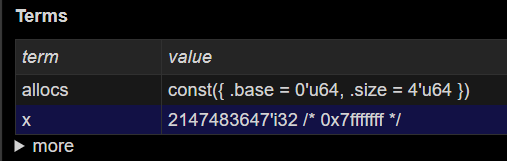
\includegraphics[width=\textwidth]{figures/increment_broken_state.png}
    \caption{Counter example for increment\_broken.c.}\label{fig:incr-broken-counter-ex}
\end{marginfigure}

We can avoid this error by constraining the values of the input with a
precondition annotation, as in \cref{fig:incr}. Here we see the keyword
\cinline{requires} is used to introduce a pre-condition on the input.
\cinline{MAXi32()} is an in-built function which represents the maximum value a
signed 32-bit integer can represent. By constraining the input so that it is
strictly less than the maximum value, the function is now guaranteed to have
no \kl{UB} for all its inputs, no matter what the context. This is because
whilst pre-conditions are \emph{assumed} inside the function, they are
\emph{required} when calling it.

\begin{marginfigure}
    \centering
    \cfile[breaklines]{code/increment.c}
    \caption{Successful signed integer increment in CN.}\label{fig:incr}
\end{marginfigure}

\begin{marginfigure}
    \ContinuedFloat*
    \centering
    \cfile[breaklines,lastline=8]{code/call_increment.c}
    \caption{Calling a signed integer increment in CN.}\label{fig:call-incr}
\end{marginfigure}

\begin{marginfigure}
    \ContinuedFloat{}
    \centering
    \cfile[breaklines,firstline=10]{code/call_increment.c}
    \caption{Calling a signed integer increment in CN.}\label{fig:call-incr-fail}
\end{marginfigure}

This is demonstrated in \cref{fig:call-incr} and \cref{fig:call-incr-fail}. In
the first, we see that from the constraint \cinline{y <=
100i32},\sidenote{Integer literals are currently written with a type
annotation, similar to Rust.} \kl{CN} deduces that \cinline[breaklines]{y <=
MAXi32()}\sidenote{As we shall see in \cref{chap:kernel-cn}, this is a
\kl{subtyping} relation, and integrating it smoothly relies on
\kl{bidirectional} type-checking.} and permits the call to \cinline{increment}.
Conversely, for the second, \cinline{INT_MAX} does not meet that constraint,
and so \kl{CN} raises an error.

\begin{marginfigure}
    \centering
    \cfile[breaklines,firstline=4]{code/decrement_broken.c}
    \caption{Failing to decrement the result of a signed integer increment in
        CN.}\label{fig:decr-broken}
\end{marginfigure}

However, if we try to decrement the result of the successful call, \kl{CN}
raises an error (\cref{fig:decr-broken}). This is because that \kl{CN} has no
indication on the constraints of the return value (other than those deduced
from its C type, namely that it fits within a signed 32-bit integer). To fix
this, we need to provide a postcondition for the function which
expresses additional constraints on the returned value (\cref{fig:decr}).

\begin{marginfigure}
    \centering
    \cfile[breaklines]{code/decrement.c}
    \caption{Successfully decrementing the result of a signed integer increment
        in CN.}\label{fig:decr}
\end{marginfigure}

To specify pointer manipulating programs, I need to introduce some new syntax.
Where in separation logic, we may say $p \mapsto v$ for arbitrary expressions
$p$ and $v$, in \kl{CN}, we restrict it so that $v$ is always a variable, akin
to $\exists{} v.\ p \mapsto v \wedge v = e$ for some expression $e$. For both
usability and technical reasons explained later (\cref{sec:friendly-syntax}), we
write this as \cninline{take v = Owned(p);}. % chktex 36

\begin{marginfigure}
    \centering
    \cfile[breaklines]{code/owned_increment.c}
    \caption{Incrementing a signed integer via a pointer in CN.}\label{fig:owned-incr}
\end{marginfigure}

This generalises to work with arrays, with syntax of the form
\cninline[breaklines,breakafter=\{=()]{take arr = each (u64 i; .. ) { Owned(p) };}, % chktex 26 chktex 37 chktex 36
called \intro{quantified} or \intro{iterated} resources, for the pre- and
postconditions of the function. \kl{CN} can also handle (in a limited, careful
fashion to preserve decidability) \intro{quantified constraints}, such as the
one in the postcondition of \cref{fig:owned-array}, to express constraints
about the elements of an array. Within the \cninline{Owned}, we express the
location with \cninline{array_shift(p,i)}, which is the specification language % chktex 36
equivalent of pointer arithmetic in \cinline{&p[i]}. Within the body of the
function, we use a \intro{CN statement}, \cninline{extract Owned<int>, 0u64;},
which acts a proof hint to \kl{CN} to tell which index of the \kl{iterated}
resource we wish to read or write from.

\begin{figure*}[tp]
    \centering
    \begin{minipage}{1.5\textwidth}
        \cfile[breaklines]{code/owned_array.c}
    \end{minipage}
    \caption{Summing up a two-element array of unsigned integers in
        CN.}\label{fig:owned-array}
\end{figure*}

\kl{Iterated} resources are powerful because they supports random access
(unlike a recursive predicate over an array, which would fix the order of
traversal).\cref{fig:init-arr-rev} shows how \kl{CN} can transform an array of
uninitialised values (\cninline{Block}s) from the precondition, into an array
of initialised values (\cninline{Owned}s) in the postcondition, by looping over
it \emph{in reverse}. All loops in \kl{CN} must be annotated with \intro{loop
invariants}, which are mostly as expected with exception of the verbose and
confusing \cninline|{_} unchanged|
syntax,\sidenote{\url{https://github.com/rems-project/cerberus/issues/443}}
which tells CN that the loop does not mutate the function arguments.

Within the loop, writing to a \cninline{Block} (or an \cninline{Owned}) transforms
it into a new \cninline{Owned}. We need two \cninline{extract}s to tell CN we
wish to first take a \cninline{Block} out of \cinline{Uninit} and then move
it into the \cninline{Init}.

\begin{figure*}[tp]
    \centering
    \begin{minipage}{1.5\textwidth}
        \cfile{code/init_array_reverse.c}
    \end{minipage}
    \caption{Initialising an array of characters in reverse in
        CN.}\label{fig:init-arr-rev}
\end{figure*}

Lastly, in the same way that separation logic predicates use $\mapsto$ as a
building block to express more complex relations between heaps and \kl{ghost}
values, \kl{CN} allows users to write \intro{resource predicate} to express
more complex relations between heaps and \kl{ghost} values.

Continuing our running example of appending two singly-linked lists of
integers, \cref{fig:append-cn} shows how one might annotate and prove such an
example in \kl{CN}. Firstly, it declares the datatype for \cninline{i32} lists,
since these are not part of \kl{CN}'s base logic. Notably, arguments to
constructors are named, not positional. After that, it declares a recursive
\cninline{[rec]} mathematical function \cninline{function} which defines what
it means to append two lists, serving the same function that $@$ did in
\cref{fig:append-annot}. The final \kl{CN} declaration is for the equivalent of
the recursive list predicate in \cref{fig:list-pred}. There are many
differences:
\begin{itemize}
    \item The \kl{CN} \cninline{predicate} looks like a function definition,
        with a signature that takes a \cninline{pointer p}, and a
        return type \cninline{(datatype seq)}, as opposed to
        $\mathrm{list}(\mathsf{p}, l)$ which has two arguments.
    \item It uses \cninline{return} statements to constrain the ghost list,
        rather than $l = \mathsf{NULL}$ or $l = {head}{:}{:}{tl}$.
    \item It uses the \cninline{take} syntax, to give names to the pointee of
        \cninline{p} (\cninline{H}) and the tail of the list \cninline{tl},
        rather than existentials $\exists{} \; {head}, \; {tl}, \mathsf{p}$.
    \item The pointee of \cninline{p} is a record \cninline{H}, with fields
        \cninline{head} and \cninline{tail} corresponding to the C struct
        fields, rather than using pointer arithmetic $\mathsf{p} + 1$.
\end{itemize}

All of these differences will be explained in more detail and justified in
\cref{sec:friendly-syntax}. I will note in passing that the syntax can also be
seen as tracing out the footprint of the heaplet containing the list, and
constructing the ghost value it represents.

For now, I will move on to the annotations on the implementation. The
precondition can be read as saying ``\emph{\cinline{IntList_append} requires
\cninline{L1} to be the ghost list constructed using \cninline{IntList}
with \cinline{xs}, and similarly for \cninline{L2} and \cinline{ys}}''. The
postcondition can be read as saying ``\emph{\cinline{IntList_append} ensures that
\cninline{L3} is a ghost list constructed using \cninline{IntList} with the
return value \cninline{return}, and \cninline{L3} is equal to \cninline{L2}
appended to \cninline{L1}}''.

Within the body of the function, in both branches of the \cinline{if}, there is
a \kl{CN statement}, this time to instruct CN to manually unfold the definition
of the recursive function at that point to aid proving the postcondition.
Conveniently, albeit
inconsistently,\sidenote{\url{https://github.com/rems-project/cerberus/issues/483}}
\kl{CN} auto-unfolds branching predicate definitions, including recursive ones,
when it is able to prove or disprove the branch conditions of that predicate,
based on the assertions in its context at a particular program point.

\begin{figure*}[tp]
    \begin{minipage}{.85\textwidth}
        \cfile[breaklines,firstline=5,lastline=24]{code/append_annot.c}
    \end{minipage}%
    \begin{minipage}{.65\textwidth}
        \cfile[breaklines,firstline=26,lastline=41]{code/append_annot.c}
    \end{minipage}
    \caption{Appending a singly-linked list of integers in CN.}\label{fig:append-cn}
\end{figure*}%

\section{Contributions of this thesis}\label{sec:contributions}

\kl{CN} has been developed by many people; my particular contributions relate
to the following subsections, which provide an overview of the remaining parts
of this thesis.

\subsection{Formalisation of \kl{CN}}

Whilst Christopher Pulte and Thomas Sewell are the primary implementers of
\kl{CN}'s \kl{proof mode}; my contributions to this part of the project have
been to clarify and formalise \kl{CN}'s theory. The end result of this work was
not only more confidence in the theoretical merits of the approach of \kl{CN},
but also clarifying its principles, and generating insights for feeding back to
the implementation.

My contributions in this part include:
\begin{itemize}
    \item A grammar of resource terms for book-keeping resource manipulations.
    \item \intro{ResCore}: A let-normal form of \kl{Cerberus}' \kl{Core} with
        reified resources.
    \item A novel, modular heap definition in a dynamic semantics for \kl{ResCore}.
    \item \intro{Kernel CN}: A formal definition of a bidirectional,
        \kl{separation logic}, \intro{refinement type} system for \kl{ResCore}.
    \item A proof of soundness of \kl{Kernel CN} with respect to the
        \kl{ResCore} dynamic semantics.
    \item A formalisation of two inference algorithms used by \kl{CN}, one for inferring
        quantifiers and one for inferring indices for \kl{iterated} predicates.
    \item A formalisation of the link between the surface syntax of \kl{CN} and
        the formal presentation in this thesis.
    \item An experience report on (a) iterating on the design of a very large type
        system using Ott~\sidecite{sewell2010ott} and (b) feeding back insights
        from the theory to the implementation.
\end{itemize}

\subsection{Design, formalisation and implementation of \kl{CN-VIP}}

In its initial version, to simplify matters, \kl{CN} was built on top of a
simple concrete \kl{memory object model}, where pointers were treated as
interchangeable with integers. However, as I briefly alluded to in
\cref{sec:c-lang}, this is not accurate with respect to how the standard and
modern compilers treat pointers. To remedy this, building on the work of
\sidetextcite{memarian2019exploring} and \sidetextcite{lepigre2022vip}, I
designed, formalised and implemented, \intro{CN-VIP}, a memory model based on
(and sound with respect to) prior work. Because of this, \kl{CN} will now
automatically check and enforce a large number of subtle rules regarding the
creation, modification and destruction of pointers and associated allocations,
at the cost of \kl{CN} becoming harder and slower to use.


My contributions in this part include:
\begin{itemize}
    \item An exploration of the design space and trade-offs when designing a
        type system for real-world memory object models.
    \item The formalisation of \kl{CN-VIP}, focusing on its modular integration into
        \kl{Kernel CN} and \kl{ResCore}.
    \item A proof of soundness of \kl{CN-VIP}, with respect to the VIP dynamic semantics.
    \item A walk-through of the implementation of \kl{CN-VIP}, along with the
        approach required to integrate it without causing pain to myself, other
        developers or users.
    \item A discussion on the problems with supporting byte-level provenance
        and round-trip casts in \kl{CN}, potential resolutions and trade-offs.
    \item A roadmap on the integration of mechanised, sound resourceful lemmas
        into \kl{CN} inspired by the design of \kl{CN-VIP}.
\end{itemize}

\subsection{Will the real world C, please stand up?}

Though it is developed inside academia, \kl{CN} is fundamentally a piece of
software, and its job is not to advance cool theory for its own sake, but to
bring a new level of assurance to \emph{existing, real-world} \kl{systems} C
code. This requires substantial engineering effort, and benefits immensely from
modern software development best practices. Though a lot of it seems obvious in
retrospect, it was not initially clear \emph{if} and \emph{when} many of
engineering challenges would become a bottleneck. I worked on three major
problems, was successful in two of them, and collaborated closely with partners
in industry looking to use \kl{CN}. As such, \kl{CN} is better poised to meet
the challenges facing any verification tool aiming to be useful outside of
academia.

My contributions in this part include:
\begin{itemize}
    \item \intro[tree-carver]{A tree carver for C}. This is Clang based tool
        which, given a C file in a large source tree, and a root file or
        functions, carves out that file and its transitive dependencies,
        including macros, for processing by other tools.
    \item \emph{An experience report}, on updating an existing proof of a \intro{buddy
        allocator} (used in the \intro{pKVM} hypervisor) to work with (a)
        bit-vectors and (b) an early version of CN-VIP\@. In particular, due to
        poor source location information, poor proof migration path and
        performance degradation, this port failed.
    \item A summary of several developer- and user-experience issues we faced,
        with reference to the their technical origin and if they exist,
        solutions.
\end{itemize}
